\documentclass[../Analysis-3.tex]{subfiles}

\begin{document}
\chapter*{Lecture 27} %Set chapter name
\addcontentsline{toc}{chapter}{Lecture 27} %Set chapter title
\setcounter{chapter}{27} %Set chapter counter
\setcounter{section}{0}
\setcounter{equation}{0}
\setcounter{figure}{0}


\section{Conservative Vector Fields}

In the previous lecture we introduced the notion of an oriented surface. For an oriented surface $S \subseteq \R^3$, we call the orientation vector field $\vec{n} : S \to \R^3$ the \textbf{normal vector field}. Now we give an example of such a vector field.

\begin{Eg}{}{}
  \begin{wrapfigure}[14]{r}{0.4\textwidth}
    \centering
    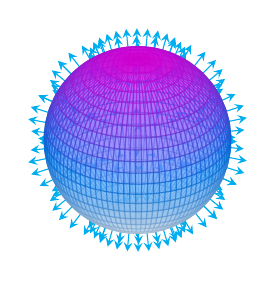
\begin{tikzpicture}
      \begin{axis}[
          width=0.85\textwidth,
          clip=false,
          hide axis,
          axis equal,
        ]
        \addplot3[
          quiver, -stealth, cyan,
          samples=15,
          variable=\a,
          variable y=\b,
          domain=0:180,
          y domain=0:360,
          quiver={
              u = {cos(a)*sin(b)},
              v = {sin(a)*sin(b)},
              w = {cos(b)},
              scale arrows=0.2,
            }
        ]({cos(a)*sin(b)}, {sin(a)*sin(b)}, {cos(b)});

        \addplot3[
          z buffer=sort,
          surf,
          samples=50,
          opacity=0.5,
          colormap/cool,
          variable=\u,
          variable y=\v,
          domain=0:180,
          y domain=0:360,
        ]({cos(u)*sin(v)}, {sin(u)*sin(v)}, {cos(v)});
      \end{axis}
    \end{tikzpicture}
    \caption{Standard normal vector field on a sphere}\label{fig1:27}
  \end{wrapfigure}
  Take $\mathbb{S}^{n-1} := \{ x \in \R^n \mid \norm{x} = 1 \}$.

  Then
  \[ \vec{n}_1(x) = x \ \forall \, x \in \mathbb{S}^{n-1} \] and
  \[ \vec{n}_2(x) = -x \ \forall \, x \in \mathbb{S}^{n-1} \]
  are the two normal vector fields on the sphere.

  \

  Generally we consider the outward normal vector, i.e., the normal vector field given by $\vec{n}_1$ as the standard normal vector field on the sphere.
\end{Eg}

\

\begin{tcolorbox}

  \begin{wrapfigure}{r}{0.4\textwidth}
    \centering
    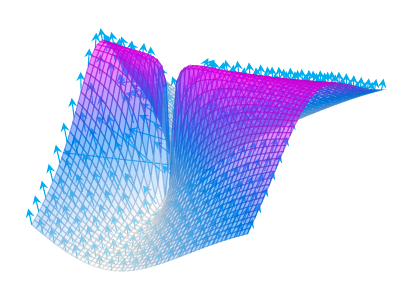
\begin{tikzpicture}
      \begin{axis}[
          hide axis, axis equal, clip = false, width = 0.7\textwidth,
        ]
        \addplot3[
          cyan, quiver, -stealth, samples=20,
          domain=-1:2, y domain = -2:2,
          quiver={
              u={(2*x*y^2)/(x^2+y^2)^2},
              v={-(2*x^2*y)/(x^2+y^2)^2},
              w={1},
              scale arrows=0.2,
            }
        ]({x},{y},{(x^2-y^2)/(x^2+y^2)});
        \addplot3[
          surf, samples=50, colormap/cool, domain=-1:2, y domain=-2:2, opacity=0.5,
        ]({x},{y},{(x^2-y^2)/(x^2+y^2)});
      \end{axis}
    \end{tikzpicture}
    \caption{Normal vector fields on a graph surface}
    \label{fig2:27}
  \end{wrapfigure}

  \textbf{Formula for Normal Vector Field.}

  Let $\mathcal{G}(f) = \qty{ (x,y,f(x,y)) \mid (x,y) \in \Op{2}}$ where $f: \Op{2} \to \R$ is a $C^1$ function. Then a parametrization of the surface $\mathcal{G}(f)$ is given by the function
  \begin{align*}
    \vec{r} : \Op{2} & \to \R^3             \\
    (x,y)            & \mapsto (x,y,f(x,y))
  \end{align*}
  Then we have
  \[
    \vec{r}_x \times \vec{r}_y = (-f_x, -f_y, 1)
  \]
  Then a normal vector field is given by
  \[
    \vec{n}(x,y) = \frac{\vec{r}_x \times \vec{r}_y}{\|\vec{r}_x \times \vec{r}_y \|}
  \]
  Unless otherwise mentioned this will be our standard orientation of the normal vector field.

\end{tcolorbox}

Usually computation of $\displaystyle\int_S \vec{F} \cdot \dd \vec{S}$ is complicated, let us look at some examples to gain more familiarity.

\begin{Eg}{}{}
  Consider the vector field $\vec{F}(x,y,z) = (x,y,z)$ on $S = \ran(r)$, where
  \[
    \vec{r}(x,y) = (\cos x, \sin x, y) \quad 0 \leq x \leq \frac{\pi}{2}, \, 0 \leq y \leq 1
  \]
  Then $\vec{r}_x \times \vec{r}_y = (\cos x, \sin x, 0)$, so $\vec{n}(x,y) = (\cos x, \sin x, 0)$ is a normal vector field.
  \begin{align*}
    \int_S \vec{F} \cdot \dd \vec{S}
     & = \int_S \vec{F} \cdot \vec{n} \dd s                                                                \\
     & = \int_0^1 \int_0^{\frac{\pi}{2}} \vec{F}(\vec{r}(x,y)) \cdot (\vec{r}_x \times \vec{r}_y) \, \dd A \\
     & = \int_0^1 \int_0^{\frac{\pi}{2}}  (\cos x, \sin x, y) \cdot (\cos x, \sin x, 0) \dd A              \\
     & = \int_0^1 \int_{0}^{\frac{\pi}{2}} \dd A                                                           \\
     & = \frac{\pi}{2}
  \end{align*}
\end{Eg}

We already know that $\displaystyle\int_{\mathcal{C}} \grad f \cdot \dd r = f(B) - f(A)$, now a natural question that arises is

\textbf{Question:} Given $\vec{F}$, does there exist $f$ a scalar field such that $\grad f = \vec{F}$ ?

\begin{Def}{Conservative Vector Field}{}
  A vector field $\vec{F}$ on $\Op{n}$ is called \textbf{conservative} if there exists a scalar field $f \in C^1(\Op{n})$ such that $\grad f = \vec{F}$, then $f$ is called the \textbf{potential function}.
\end{Def}

\begin{Thm}{}{27:1}
  Let $\vec{F}$ be a vector field over $\Op{n}$, the following are equivalent:
  \begin{enumerate}
    \item $\vec{F}$ is conservative.
    \item $\displaystyle\int_{\mathcal{C}}\vec{F} \cdot \dd r = 0$, for all closed and piecewise smooth curve $\mathcal{C}$.
    \item $\displaystyle\int_{\mathcal{C}_1} \vec{F} \cdot \dd r = \int_{\mathcal{C}_2} \vec{F} \cdot \dd r$, for all curves $\mathcal{C}_1$ and $\mathcal{C}_2$ with same initial and end points.
  \end{enumerate}
\end{Thm}

\textbf{Question:} Given a vector field $\vec{F}$, can we conclude $\vec{F}$ is conservative? (NO!)

We will give a general picture for the most common case, when $n = 3$. Let $\vec{F} = (P,Q,R)$ where $P,Q,R$ are scalar fields. Now if $\vec{F} = \grad f$ for some scalar field $f$, then we would have
\begin{align}\label{eq1:27}
   & f_x \equiv \pdv{f}{x} = P \nonumber \\
   & f_y \equiv \pdv{f}{y} = Q           \\
   & f_z \equiv \pdv{f}{z} = R \nonumber
\end{align}
Then we can define \textbf{curl} of a vector field
\[
  \curl \vec{F} := \begin{vmatrix}
    \hat{i}   & \hat{j}   & \hat{k}   \\
    \pdv{}{x} & \pdv{}{y} & \pdv{}{z} \\
    P         & Q         & R
  \end{vmatrix}
\]
Then expanding this out and using the relations (\ref{eq1:27}) and others we get that $\curl \vec{F} = 0$. So, we have proved that if $\vec{F}$ is conservative then $\curl \vec{F} = 0$.

\

\textbf{Remark.} Thus, a necessary condition for a vector field to be conservative is that, its curl should be the zero vector field.

\

\begin{Eg}{}{}
  Let $\vec{F}(x,y) = (y-3,x+2) = (P,Q)$ (say), then $\pdv{P}{y} = \pdv{Q}{x} = 1$. Let $f$ be a possible potential function, then
  \[
    \pdv{f}{x} = y-3 \quad \mbox{ and } \quad \pdv{f}{y} = x+2
  \]
  Then by \textbf{Fundamental Theorem of Calculus} (assuming domain is convex) we get
  \[
    f(x,y) = xy - 3x + g(y)
  \]
  But then using $\pdv{f}{y} = x+2$ we get
  \[
    x + g'(y) = \pdv{f}{y} = x+2 \Rightarrow g'(y) = 2
  \]
  Therefore taking $f(x,y) = xy - 3x + 2y$ gives us a potential function for the vector field $\vec{F}$.
\end{Eg}


\textbf{Remark.} This approach works for all $\vec{F}$ such that $\curl \vec{F} = 0$ and the domain is convex.

\begin{Eg}{}{}
  Let $\vec{F}(x,y) = \left( \frac{-y}{x^2+y^2}, \frac{x}{x^2+y^2} \right) = (P,Q)$ (say) on $\R^2 \setminus \{0\}$. Then we have $\pdv{P}{y} = \pdv{Q}{x}$, but we will show that $\vec{F}$ is not conservative. Consider the curve
  \[
    \mathcal{C} : \gamma(t) = ( \cos t, \sin t), \quad 0 \leq t \leq 2\pi
  \]
  then
  \begin{align*}
    \int_{\mathcal{C}} \vec{F} \cdot \dd r
     & = \int_0^{2\pi}  \vec{F}(\gamma(t))\cdot \gamma'(t) \, \dd t        \\
     & = \int_0^{2\pi}  (-\sin t, \cos t) \cdot (-\sin t, \cos t) \, \dd t \\
     & = \int_0^{2\pi} \dd t                                               \\
     & = 2\pi
  \end{align*}
  But $\mathcal{C}$ is clearly a closed curve, hence by Theorem \ref{th:27:1} we must have $\displaystyle\int_{\mathcal{C}} \vec{F} \cdot \dd r = 0$. (Contradiction!)
\end{Eg}

\section{Green's Theorem}

\begin{Def}{Simply Connected Domain}{}
  Let $\mathcal{D}$ be an open and connected set. Let $\mathcal{C}$ be a simple and closed curve if $\mathcal{C}$ can be shrunk continuously to a point inside $\mathcal{D}$, then we say $\mathcal{D}$ is \textbf{simply connected}.
\end{Def}

\begin{figure}[h]
  \centering
  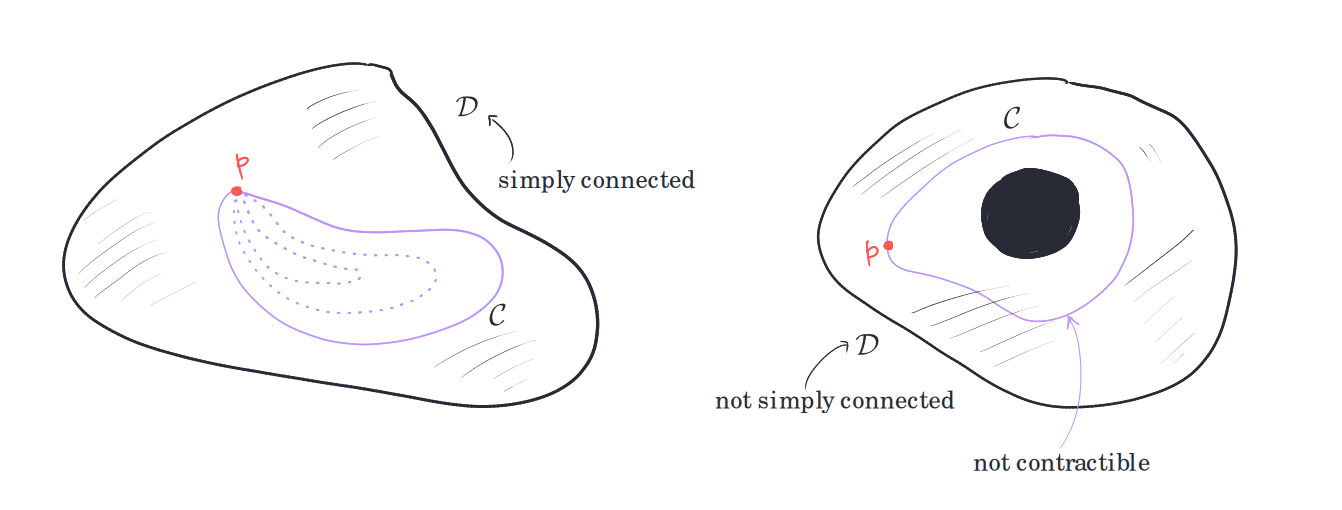
\includegraphics[width=\textwidth]{../figures/lec27.4.png}
  \caption{Examples of simply connected and not simply connected region}
  \label{fig4:27}
\end{figure}

\begin{Thm}{Green's Theorem}{green}
  Let $\mathcal{R} \subseteq \R^2 $ be a simply connected domain with boundary curve $\mathcal{C}$ where parametrization is taken in anti-clockwise direction. Let $\vec{F} = (P,Q)$ be a $C^1$ vector field on $\mathcal{R}$, then
  \[
    \int_{\mathcal{C}} \vec{F} \cdot \dd r := \int_{\mathcal{C}} P \, \dd x + Q \, \dd y = \int_{\mathcal{R}} \left( \pdv{Q}{x} - \pdv{P}{y}\right) \dd A
  \]
\end{Thm}

What happens when $\mathcal{R}$ is not simply connected?
\begin{figure}[H]
  \centering
  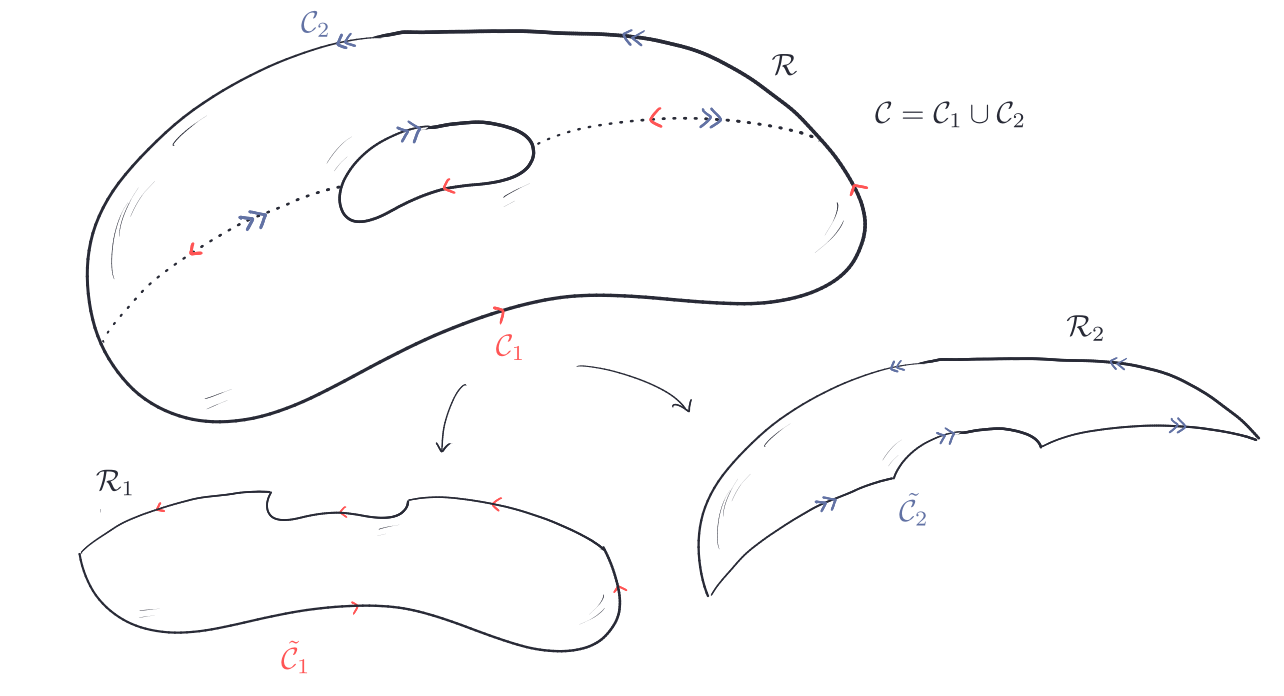
\includegraphics[width=0.8\textwidth]{../figures/lec27.5.png}
  \caption{You break up the region $\mathcal{C}$ with the hole into two regions without holes $\mathcal{C}_1$ and $\mathcal{C}_2$.}
  \label{fig5:27}
\end{figure}
\begin{align*}
  \int_{\mathcal{C}} P \, \dd x + Q \, \dd y
   & = \int_{\tilde{\mathcal{C}}_1} P \, \dd x + Q \, \dd y + \int_{\tilde{\mathcal{C}}_2} P \, \dd x + Q \, \dd y \\
   & = \int_{\mathcal{R}_1} (Q_x - P_y) \, \dd A + \int_{\mathcal{R}_2} (Q_x - P_y) \, \dd A                       \\
   & = \int_{\mathcal{R}} (Q_x - P_y) \, \dd A
\end{align*}


\end{document}
